%###########################################################################
%
% Anhang
%
%###########################################################################
%\begin{appendix}
%\label{chap:Appendix}
%\chapter{Appendix A}
%\setcounter{chapter}{1}
%\addcontentsline{toc}{chapter}{Appendix}
%###########################################################################
% Anhang A
%###########################################################################
%\label{A}
%....


%\chapter{Appendix B}
%###########################################################################
% Anhang B
%###########################################################################
%\label{B}

%\pagebreak
%###########################################################################
%\end{appendix}

\renewcommand\thesection{\Alph{section}}
\renewcommand\thefigure{\thesection\arabic{figure}}
\renewcommand{\thetable}{\thesection\arabic{table}}
\setcounter{figure}{0}
\setcounter{table}{0}
\setcounter{section}{0}

\chapter*{Appendix}
\addcontentsline{toc}{chapter}{Appendix}

\label{chap:Appendix}

%-------------------------------------------------
\section{Thermal Controls System} \label{sec:AppendixThermal}
%-------------------------------------------------
\subsection{Heat energy eqilibrium}

\underline{RTG:}
\[ \dot{Q}_{} = 0  \]\\[2em]

% \dot{Q}_{}
\underline{Electric Bay:}
\[ \dot{Q}_{B,intern}+ CON1 \cdot (T_{RTG}-T_{Bay})+ CON3 \cdot (T_{Chassis}-T_{Bay})  -\epsilon_{alloy}\cdot \sigma_b \cdot S_{Bay}\cdot T_{Bay}^4=0 \]
with: 
\[\dot{Q}_{B,intern} = \dot{Q}_{C\&DH} + \dot{Q}_{Tranceiver} +\dot{Q}_{Receiver} +\dot{Q}_{PCDU} \] \\[2em]

\underline{Drill \& Analyser:}
\[ \dot{Q}_{} = 0  \]\\[2em]

\underline{Camera:}
\[ \dot{Q}_{} = 0  \]\\[2em]

\underline{Radiator:}
\[ \dot{Q}_{} = 0  \]\\[2em]

\underline{Chassis:}
\[ \dot{Q}_{} = 0  \]\\[2em]

\underline{Steer Enine:}
\[ \dot{Q}_{} = 0  \]\\[2em]

\underline{Distribution Node 1:}
\[ \dot{Q}_{} = 0  \]\\[2em]

\underline{Drive Engine:}
\[ \dot{Q}_{} = 0  \]\\[2em]

\underline{Distribution Node 1:}
\[ \dot{Q}_{} = 0  \]\\[2em]


\subsection{Heat conductance}


\subsection{Values}
\begin{table}[htb]
	\centering
	\begin{tabular}{lcc}
		\hline
		 & \multicolumn{2}{l}{Temperature limits in [$^\circ C$]} \\ 
		Component	&	min. & max. \\\hline
		Command \& Data Handling & & \\
		Transmitter & -10 & 50 \\
		Receiver & -30 & 70 \\
		PCDU & -40 & 60 \\
		Battery & -35 & 60 \\
		Camera & -40 & 70 \\
		Objektive  & -40 & 71 \\
		Steering Engine & -30 & 100 \\
		Steering Gear & -30 & 85 \\
		Drive Engine & -40 & 100 \\
		Drive Gear & -40 & 100 \\ \hline
	\end{tabular}
	\caption{Temperatur limits of the rover components.}
	\label{tab:tsc_limits}
\end{table}

\begin{table}[htb]
	\centering
	\begin{tabular}{lccccc}
		\hline
		& \multicolumn{2}{l}{Emisivity [-]} & \multicolumn{2}{l}{Absorptivity [-]}& Source  \\ 
		Surface finishing	&	min. & max. 	&	min. & max.  & \\\hline
		Sand blasted alloy & & & & & \\
		White paint & & & & & \\
	\end{tabular}
	\caption{Minimum and maximum of surface emisivity and absorptivity values.}
	\label{tab:tsc_surface}
\end{table}




\section{Radiation}
\label{sec:AppendixRadiation}

All calculations and figures in \autoref{sec:AppendixRadiation} are performed with SPENVIS unless otherwise stated.

%TODO welche Tools verwendet und welchen Orbit zum simulieren
%TODO letzte Schicht Si
%TODO slap statt squere ausgewählt wegen Eis
%TODO wieviel mm von welchem Material

\begin{figure}[htb]
     \centering
     \begin{subfigure}[b]{0.49\textwidth}
         \centering
         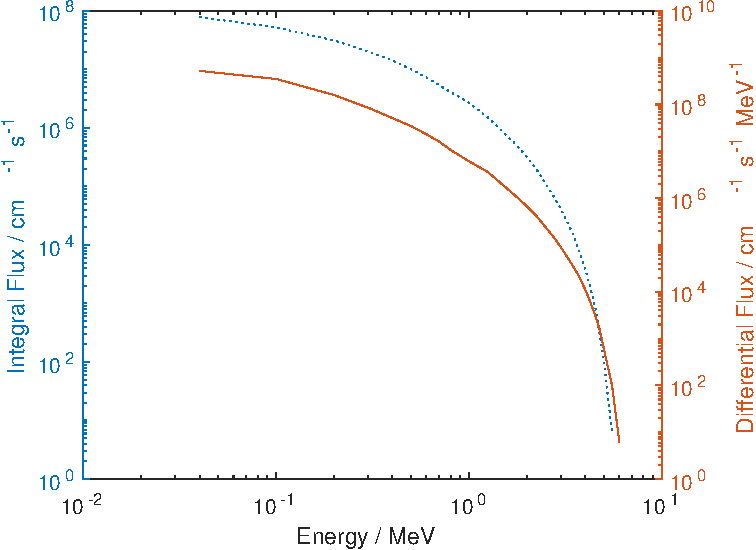
\includegraphics[width=\textwidth]{Media/E_Electron_Flux}
         \caption{Average spectra of trapped electrons around Earth}
         \label{fig:trappedelectronsEarth}
     \end{subfigure}
     \hfill
     \begin{subfigure}[b]{0.49\textwidth}
         \centering
         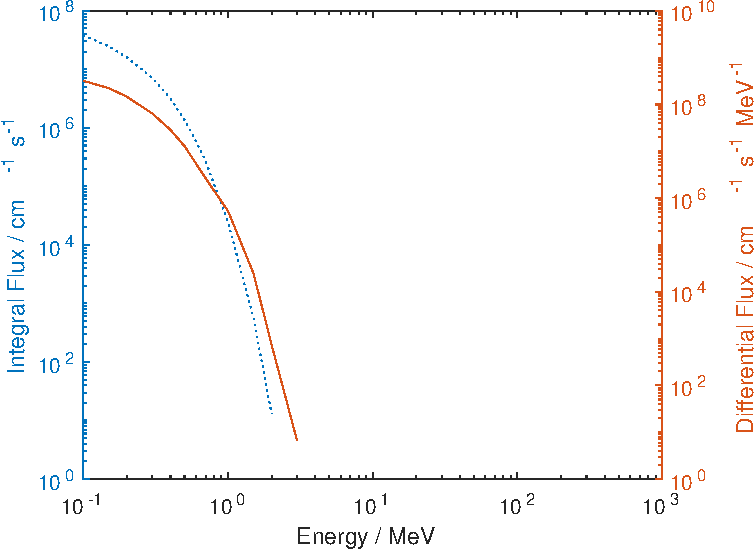
\includegraphics[width=\textwidth]{Media/E_Proton_Flux}
         \caption{Average spectra of trapped protons around Earth}
         \label{fig:trappedprotonsEarth}
     \end{subfigure}
     \hfill
     \begin{subfigure}[b]{0.49\textwidth}
         \centering
         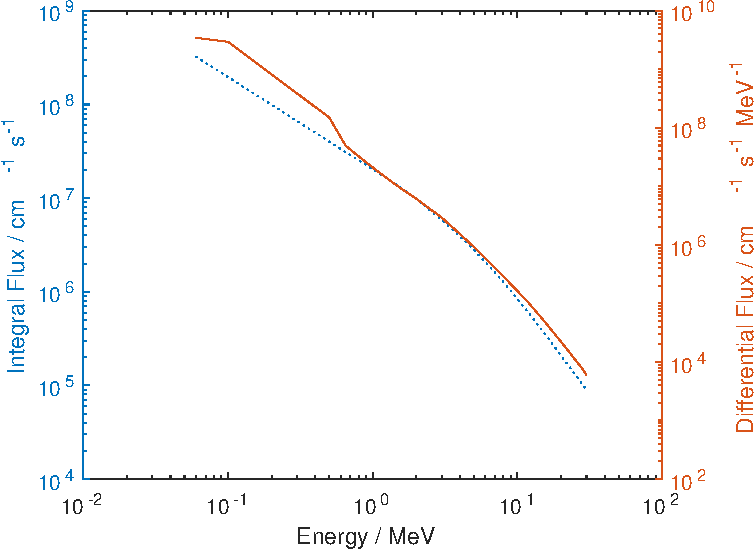
\includegraphics[width=\textwidth]{Media/J_Electron_Flux}
         \caption{Average spectra of trapped electrons around Jupiter}
         \label{fig:trappedelectronsJupiter}
     \end{subfigure}
     \hfill
     \begin{subfigure}[b]{0.49\textwidth}
         \centering
         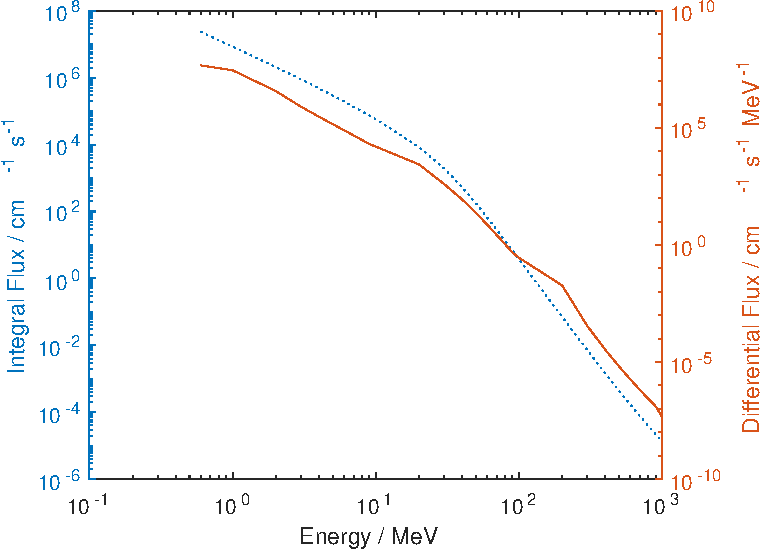
\includegraphics[width=\textwidth]{Media/J_Proton_Flux}
         \caption{Average spectra of trapped protons around Jupiter}
         \label{fig:trappedprotonsJupiter}
     \end{subfigure}
     \caption{Average trapped proton and electron fluxes on an orbit around earth at 25,000 km, through the outer Van Allen radiation belt, and on Europa's orbit around Jupiter.}
     \label{fig:trappedprotonelectronfluxes}
\end{figure}

\begin{figure}[htb]
     \centering
     \begin{subfigure}[b]{0.49\textwidth}
         \centering
         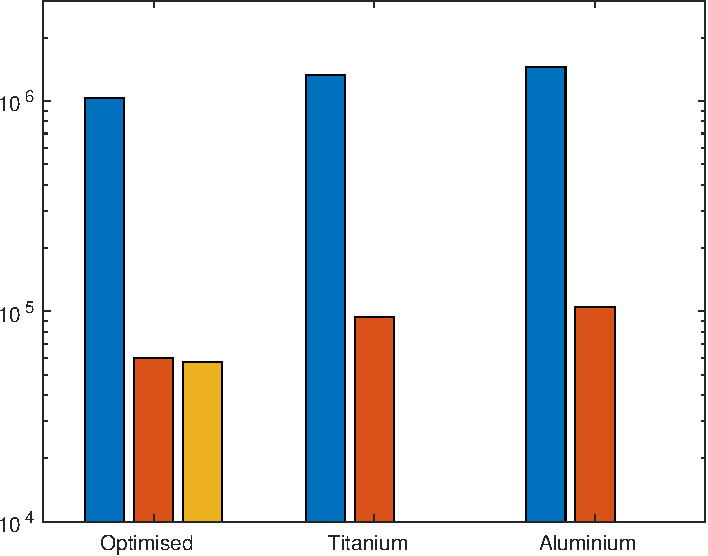
\includegraphics[width=\textwidth]{Media/J_Electron_Shielding}
         \caption{TID for Electrons as Source Particles}
         \label{fig:TIDElectronShielding}
     \end{subfigure}
     \hfill
     \begin{subfigure}[b]{0.49\textwidth}
         \centering
         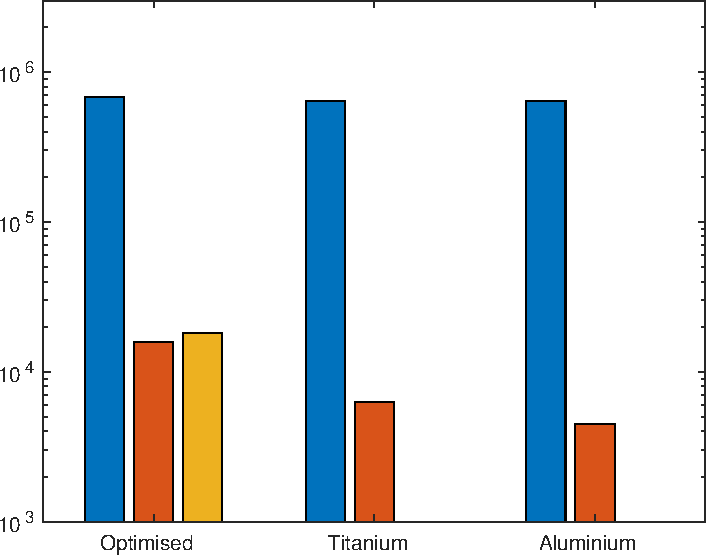
\includegraphics[width=\textwidth]{Media/J_Proton_Shielding}
         \caption{TID for Proton as Source Particles}
         \label{fig:TIDProtonShielding}
     \end{subfigure}
     \caption{TID of aluminium, titanium, and the optimised radiation structure shown in \autoref{tab:OptimalRadiationProtection} with an weight target of 0.5 \(\text{g/cm}^2\) over 30 days of exposure on Europa}
     \label{fig:AluminiumTitanOptimised}
\end{figure}

\begin{table}[htb]
\centering
\caption{Used components and the respective radiation tolerance and location}
\begin{adjustbox}{max width=\textwidth}
\begin{tabular}[l]{lccccc}

	\toprule
		Components	&	Rated TID	&	Exposed TID	&	Location\\
	\midrule
	
	Electric Motors	&	-	&	< 205 krad	&	locomotion housing\\	
	
	Harness	&	-	&	< 98 krad	&	chassis\\	
	
	Stereo Vision Cams	&	40	&	< 31 krad	&	camera housing\\	
	
	OBC	&	1000	&	< 17 krad	&	E-Bay\\
	
	PCDU	&	20	&	< 17 krad	&	E-Bay\\
	

	\bottomrule

\end{tabular}
\end{adjustbox}
\label{tab:RadiationList}
\end{table}

\begin{figure}[htb]
     \centering
     \begin{subfigure}[b]{0.49\textwidth}
         \centering
         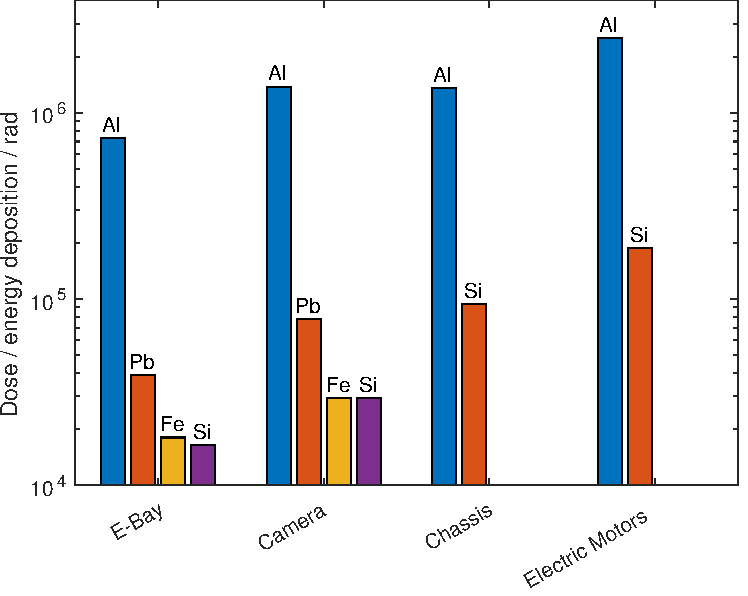
\includegraphics[width=\textwidth]{Media/J_Electron_Compartments}
         \caption{TID for Electrons as Source Particles for different compartments}
         \label{fig:TIDElectronShielding}
     \end{subfigure}
     \hfill
     \begin{subfigure}[b]{0.49\textwidth}
         \centering
         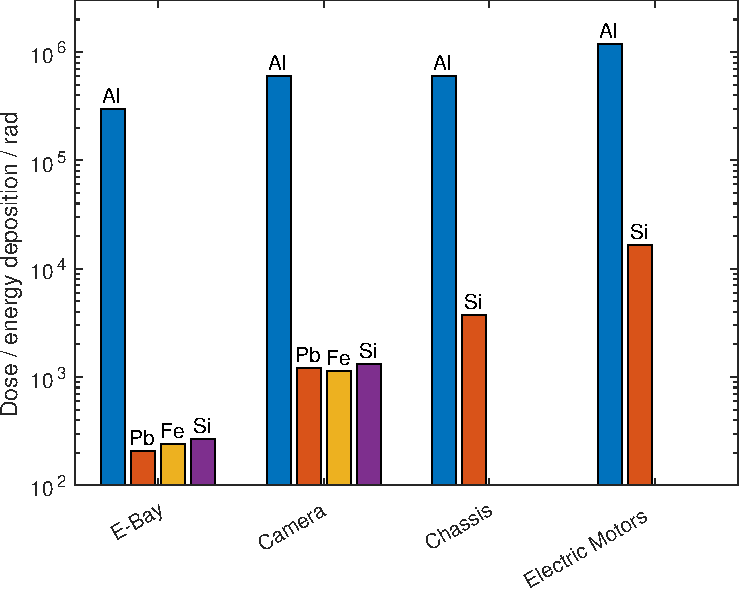
\includegraphics[width=\textwidth]{Media/J_Proton_Compartments}
         \caption{TID for Proton as Source Particles for different compartments}
         \label{fig:TIDProtonShielding}
     \end{subfigure}
     \caption{TID for different compartments}
     \label{fig:CompartmentTID}
\end{figure}

\clearpage

\section{Appendix 2}
\label{sec:Appendix2}

...

\cleardoublepage